\documentclass[a4paper,12pt]{article}

\usepackage{../usfdvl}


\title{Project 3: Gift Wrapping Convex Hulls}
\SetDocumentFooter{}{}


\begin{document}

\maketitle

\section{Objectives}

\myparagraph{In this assignment you will implement the 'easiest' of the convex hull algorithms.}


\projectGroundRules


\vspace{5pt}
\section{Assignment Instructions}

\begin{itemize}

\item Download the provided skeleton code and complete the unfinished functions in \texttt{ConvexHull.pde}.

\begin{itemize}

   \item \texttt{Polygon ConvexHullGiftWrapped( ArrayList<Point> points )} --- Takes in a list of points and returns a polygon that should be the convex hull of the points.
   
\end{itemize}

\item To test your code the Processing skeleton provided gives visual feedback for creating random point sets and testing your capabilities.

\end{itemize}

\begin{center}
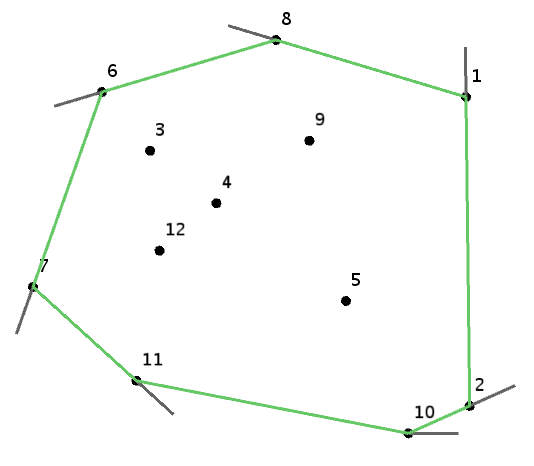
\includegraphics[width=8cm]{../images/project3.png}
\end{center}

\projectSubmission



\end{document}
